\clearpage

\chapter{Results and Discussion}

In this chapter, we present the outcomes of our experiments, encompassing both quantitative
evaluations and comparative analyses across different model configurations. The aim
is to assess the effectiveness of PQG using language models fine-tuned with parameter-efficient
techniques such as LoRA and quantized via the NF4 format. Quantitative metrics—namely
Perplexity, BLEU, METEOR, and BERTScore—are employed to evaluate
both the linguistic fluency and semantic accuracy of the generated quests. These metrics
are reported across baseline and fine-tuned versions of selected models to capture
improvements attributable to our training pipeline.

Beyond numerical evaluations, we also explore model behavior through comparative
analysis to highlight strengths, weaknesses, and trade-offs between performance and efficiency.
This includes assessing how quantization impacts output quality and whether
LoRA-based adaptation leads to better task-specific generalization.

Finally, we provide an interpretative discussion contextualizing these results within
the broader scope of the project, including reflections on the utility of automated metrics,
qualitative patterns observed in generated samples, and practical implications for future
applications in game development.

\section{Training Results}

\begin{table}[t]
  \centering
  \scriptsize
  \renewcommand{\arraystretch}{1.3}
  \begin{tabularx}{0.95\textwidth}{
    >{\raggedright\arraybackslash}p{5cm}
    >{\centering\arraybackslash}X
    >{\centering\arraybackslash}X
    >{\centering\arraybackslash}X
    >{\centering\arraybackslash}X
  }
    \toprule
    \textbf{Model} & \textbf{Final Train Loss} & \textbf{Eval Loss} & \textbf{Max Grad Norm} & \textbf{Min Grad Norm} \\
    \midrule
    GPT-2 & 2.4868 & 2.1573 & 0.6707 & 0.2780 \\
    GPT-2 Medium & 2.1188 & 1.8826 & 0.4840 & 0.2307 \\
    GPT-2 Large & 1.6781 & 1.5232 & 0.4557 & 0.2274 \\
    LLaMA-3.2-1B-Instruct & 1.8126 & 1.6759 & 1.9814 & 1.0357 \\
    TinyLLaMA-1.1B-Chat-v1.0 & \textbf{1.3555} & \textbf{1.2684} & 2.5458 & 1.0018 \\
    \bottomrule
  \end{tabularx}
  \caption{Training and evaluation metrics reported for each fine-tuned model}
  \label{table:training-results}
\end{table}

\begin{figure}[t]
  \centering
  \begin{subfigure}[t]{0.48\textwidth}
    \centering
    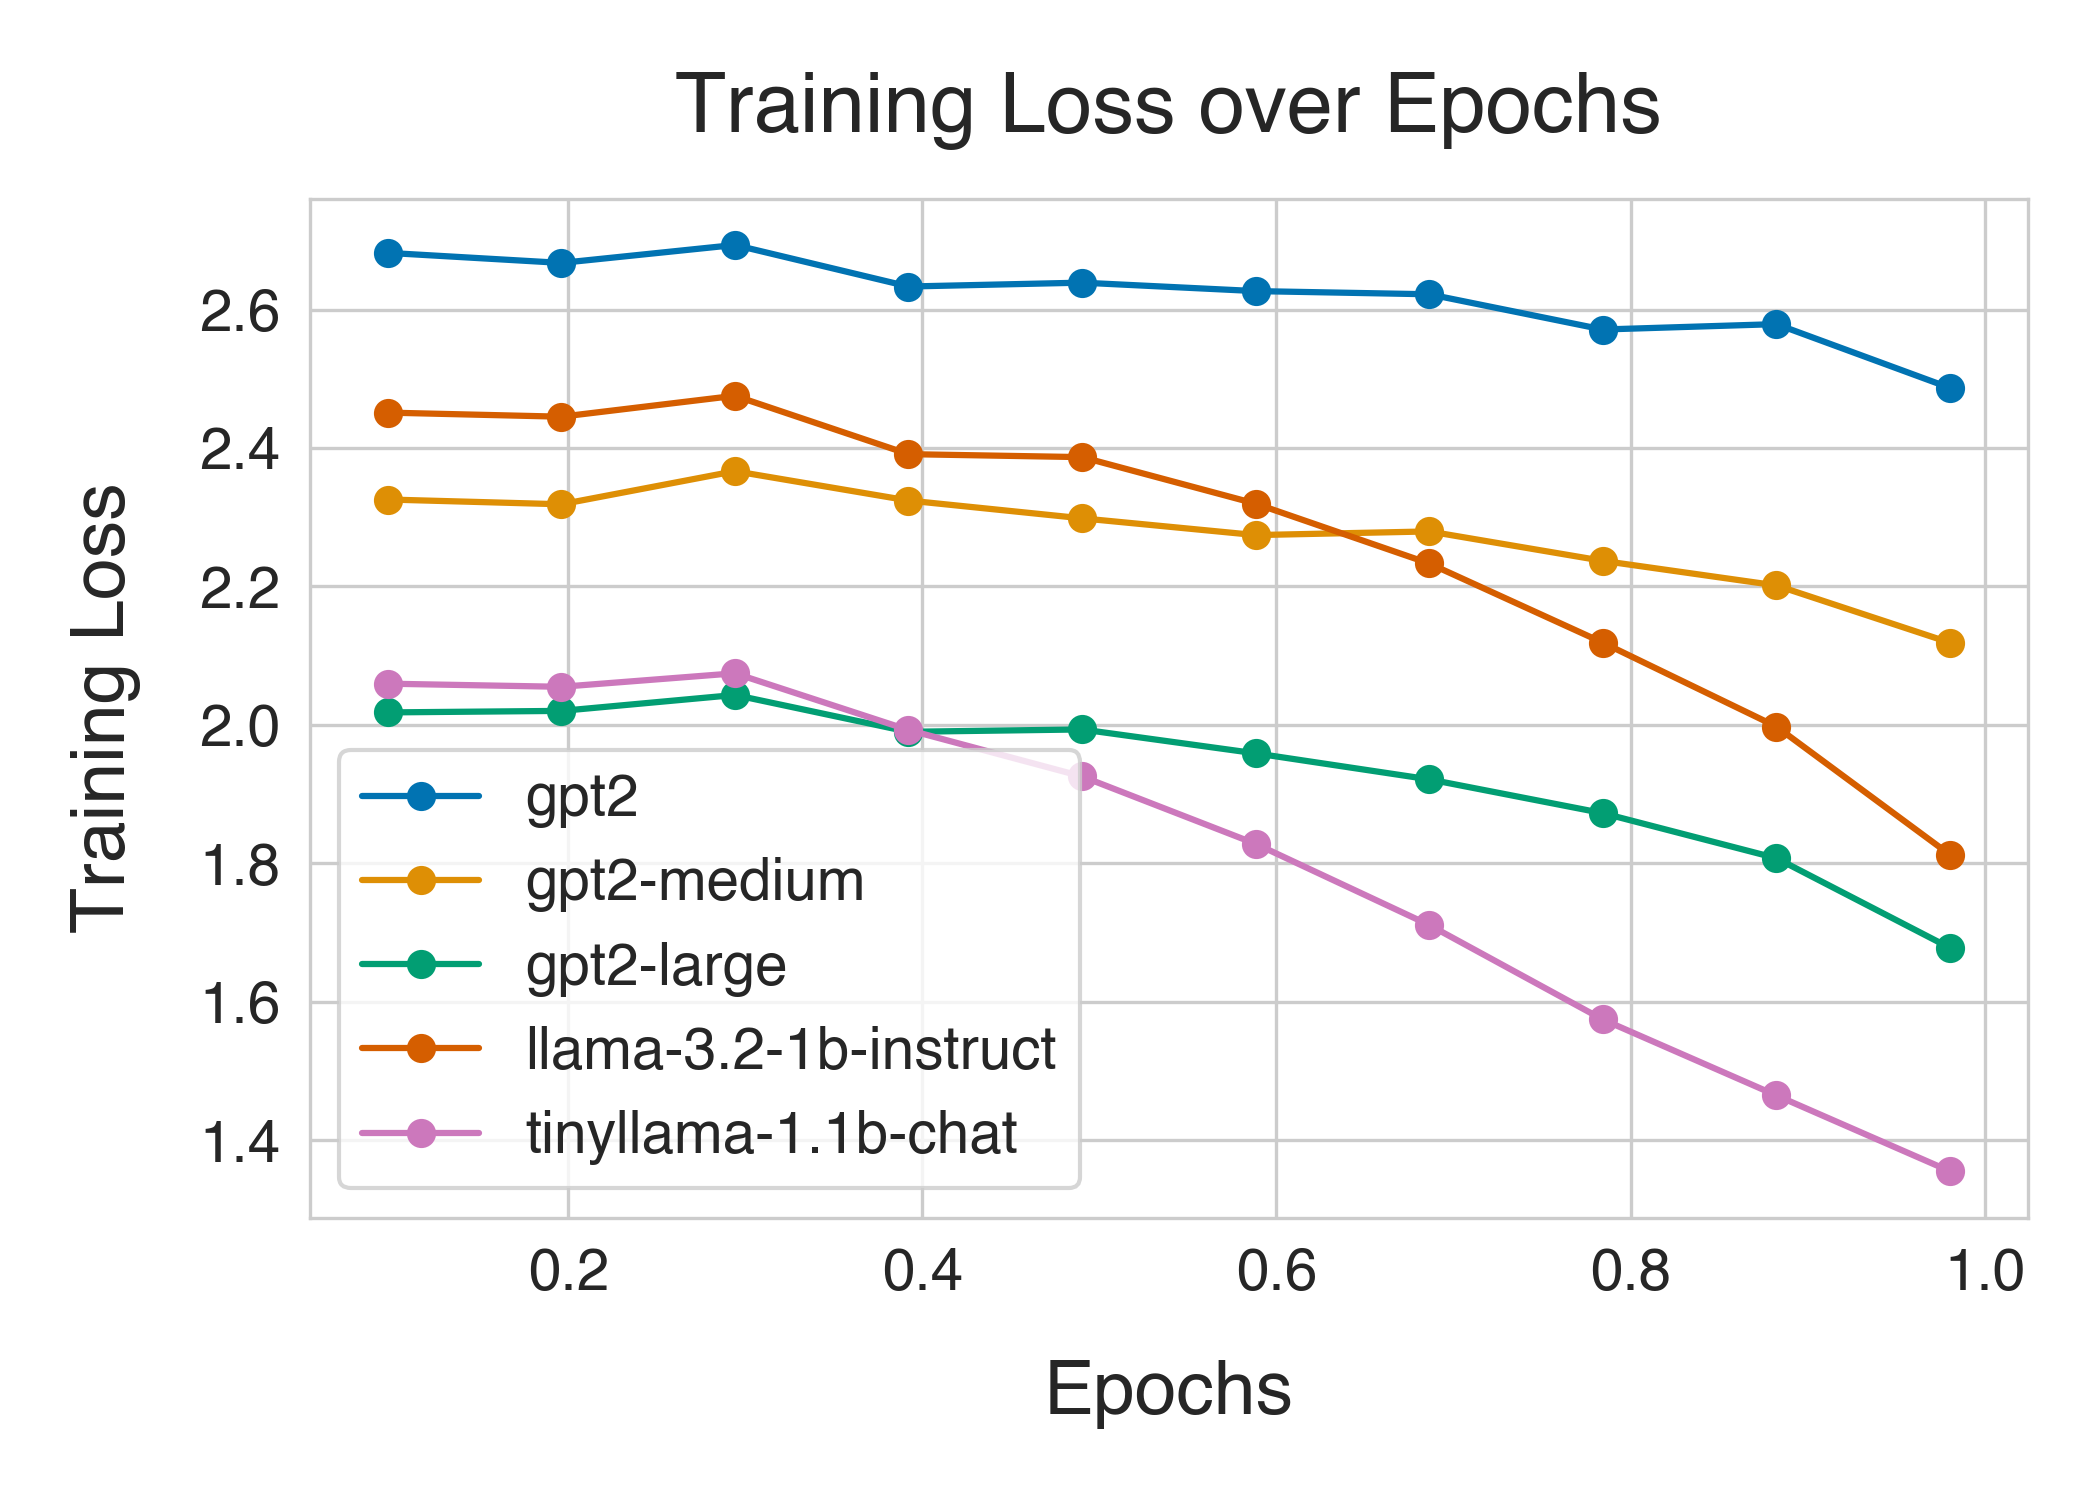
\includegraphics[width=\textwidth]{training_train_losses.png}
    \caption{Training loss over epochs. Lower final loss indicates better convergence; sharp early declines reflect faster initial learning.}
    \label{fig:train-loss}
  \end{subfigure}
  \hfill
  \begin{subfigure}[t]{0.48\textwidth}
    \centering
    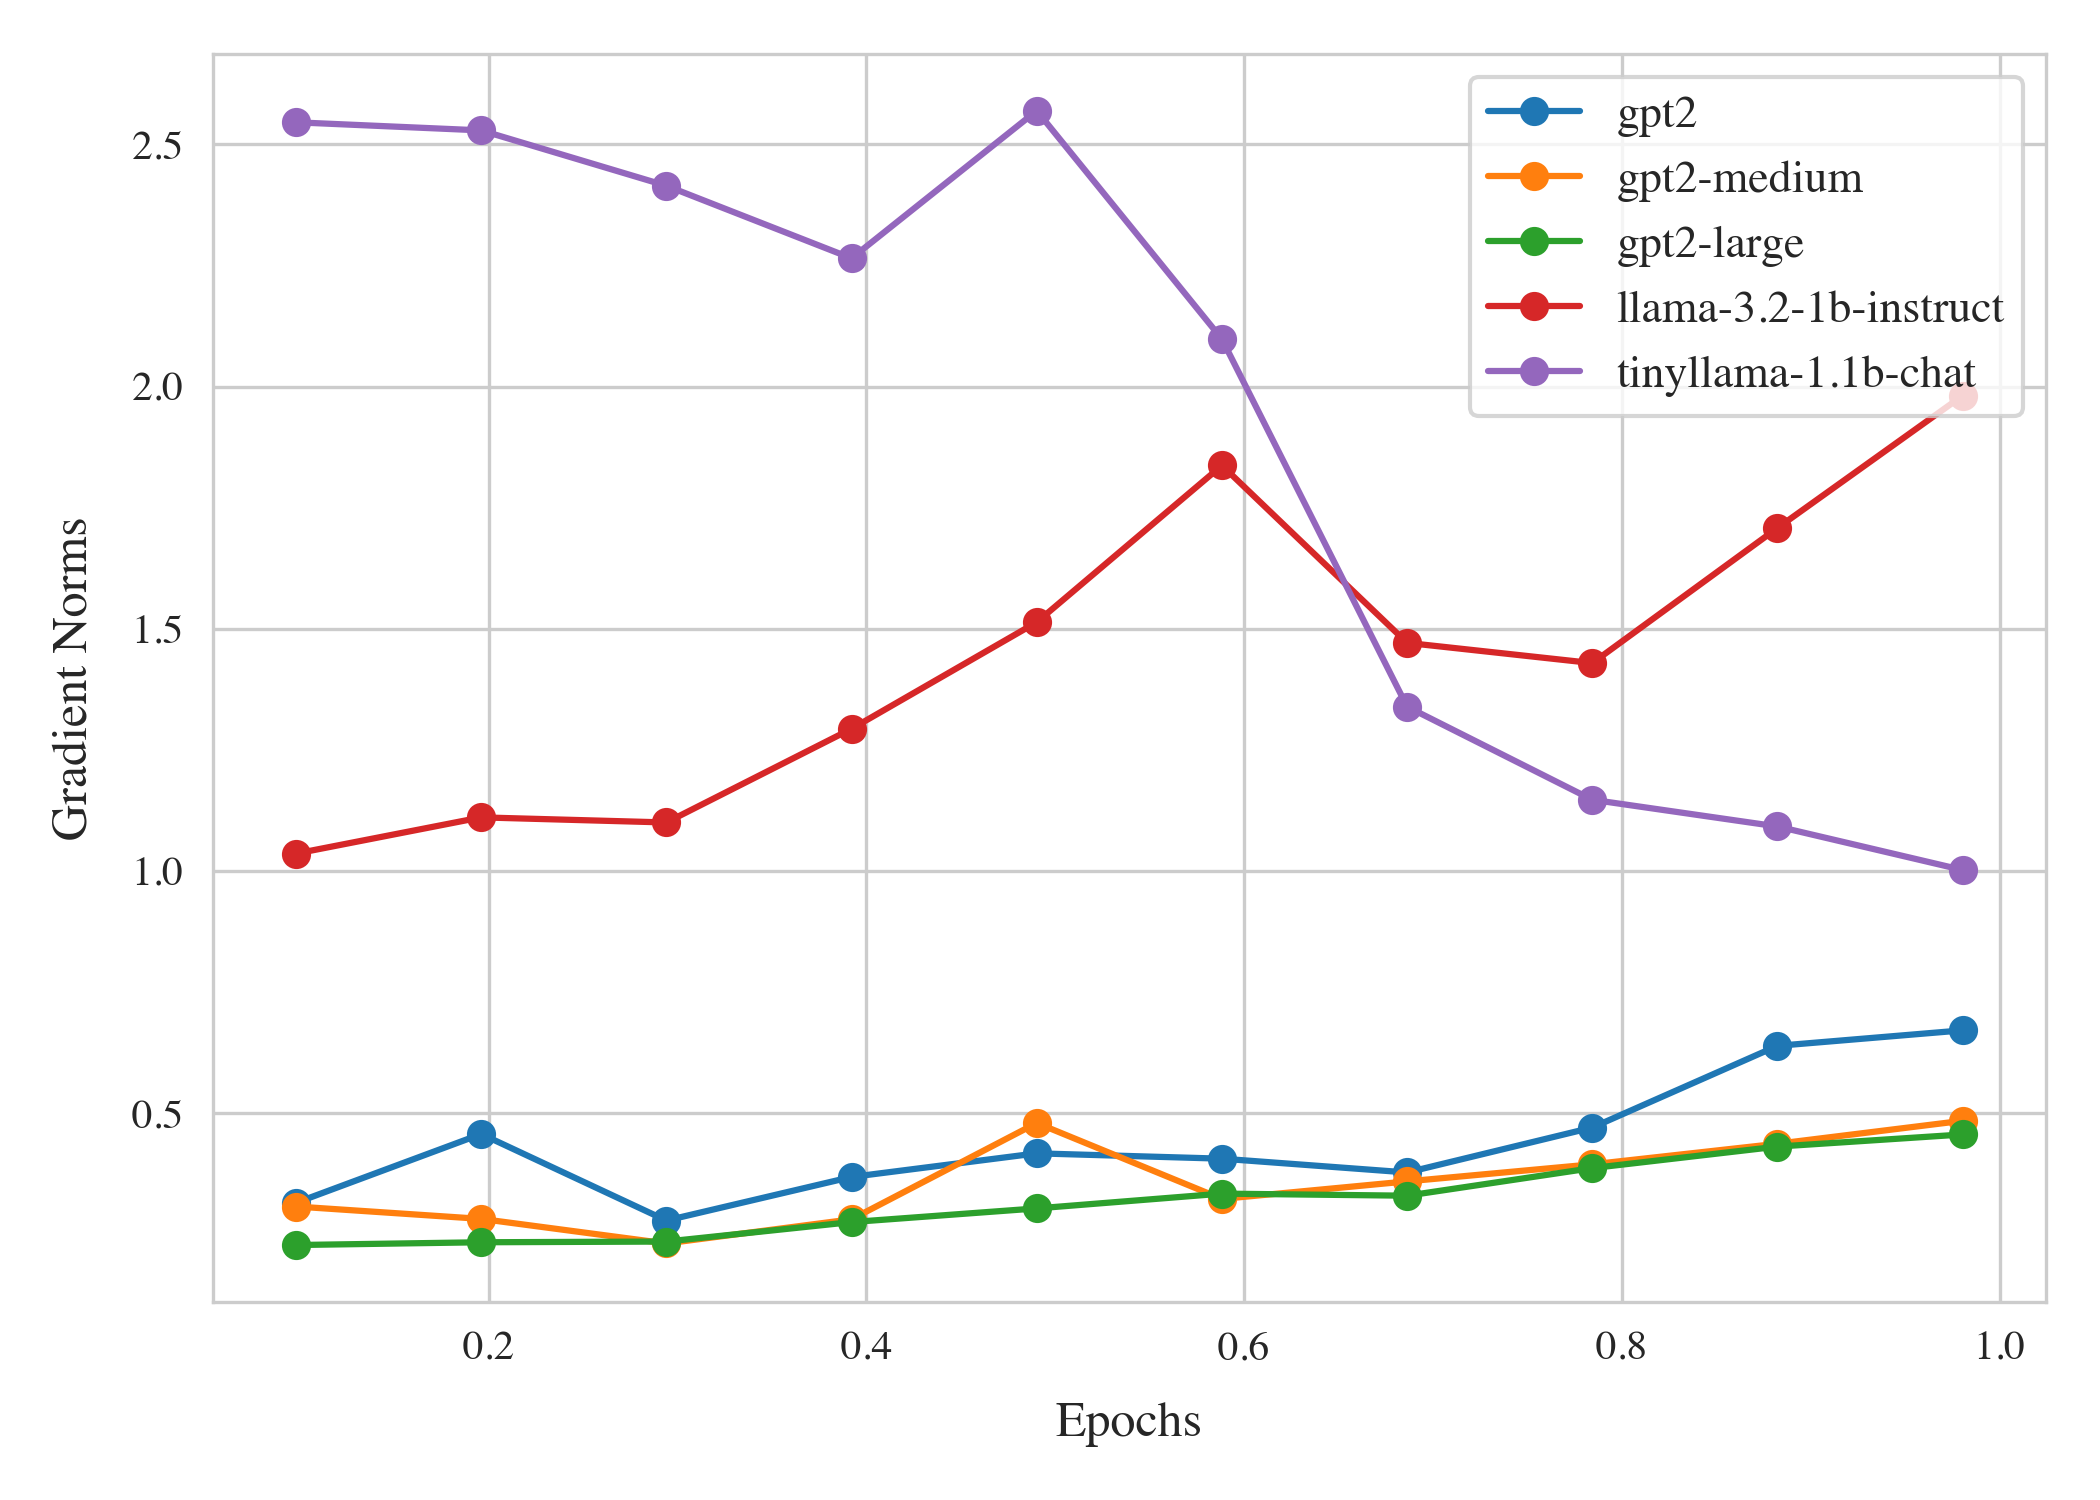
\includegraphics[width=\textwidth]{training_grad_norms.png}
    \caption{Gradient norm values. Stable norms imply smooth optimization; spikes may reflect instability or poor learning rate settings.}
    \label{fig:grad-norms}
  \end{subfigure}
  \vskip\baselineskip
  \begin{subfigure}[t]{0.48\textwidth}
    \centering
    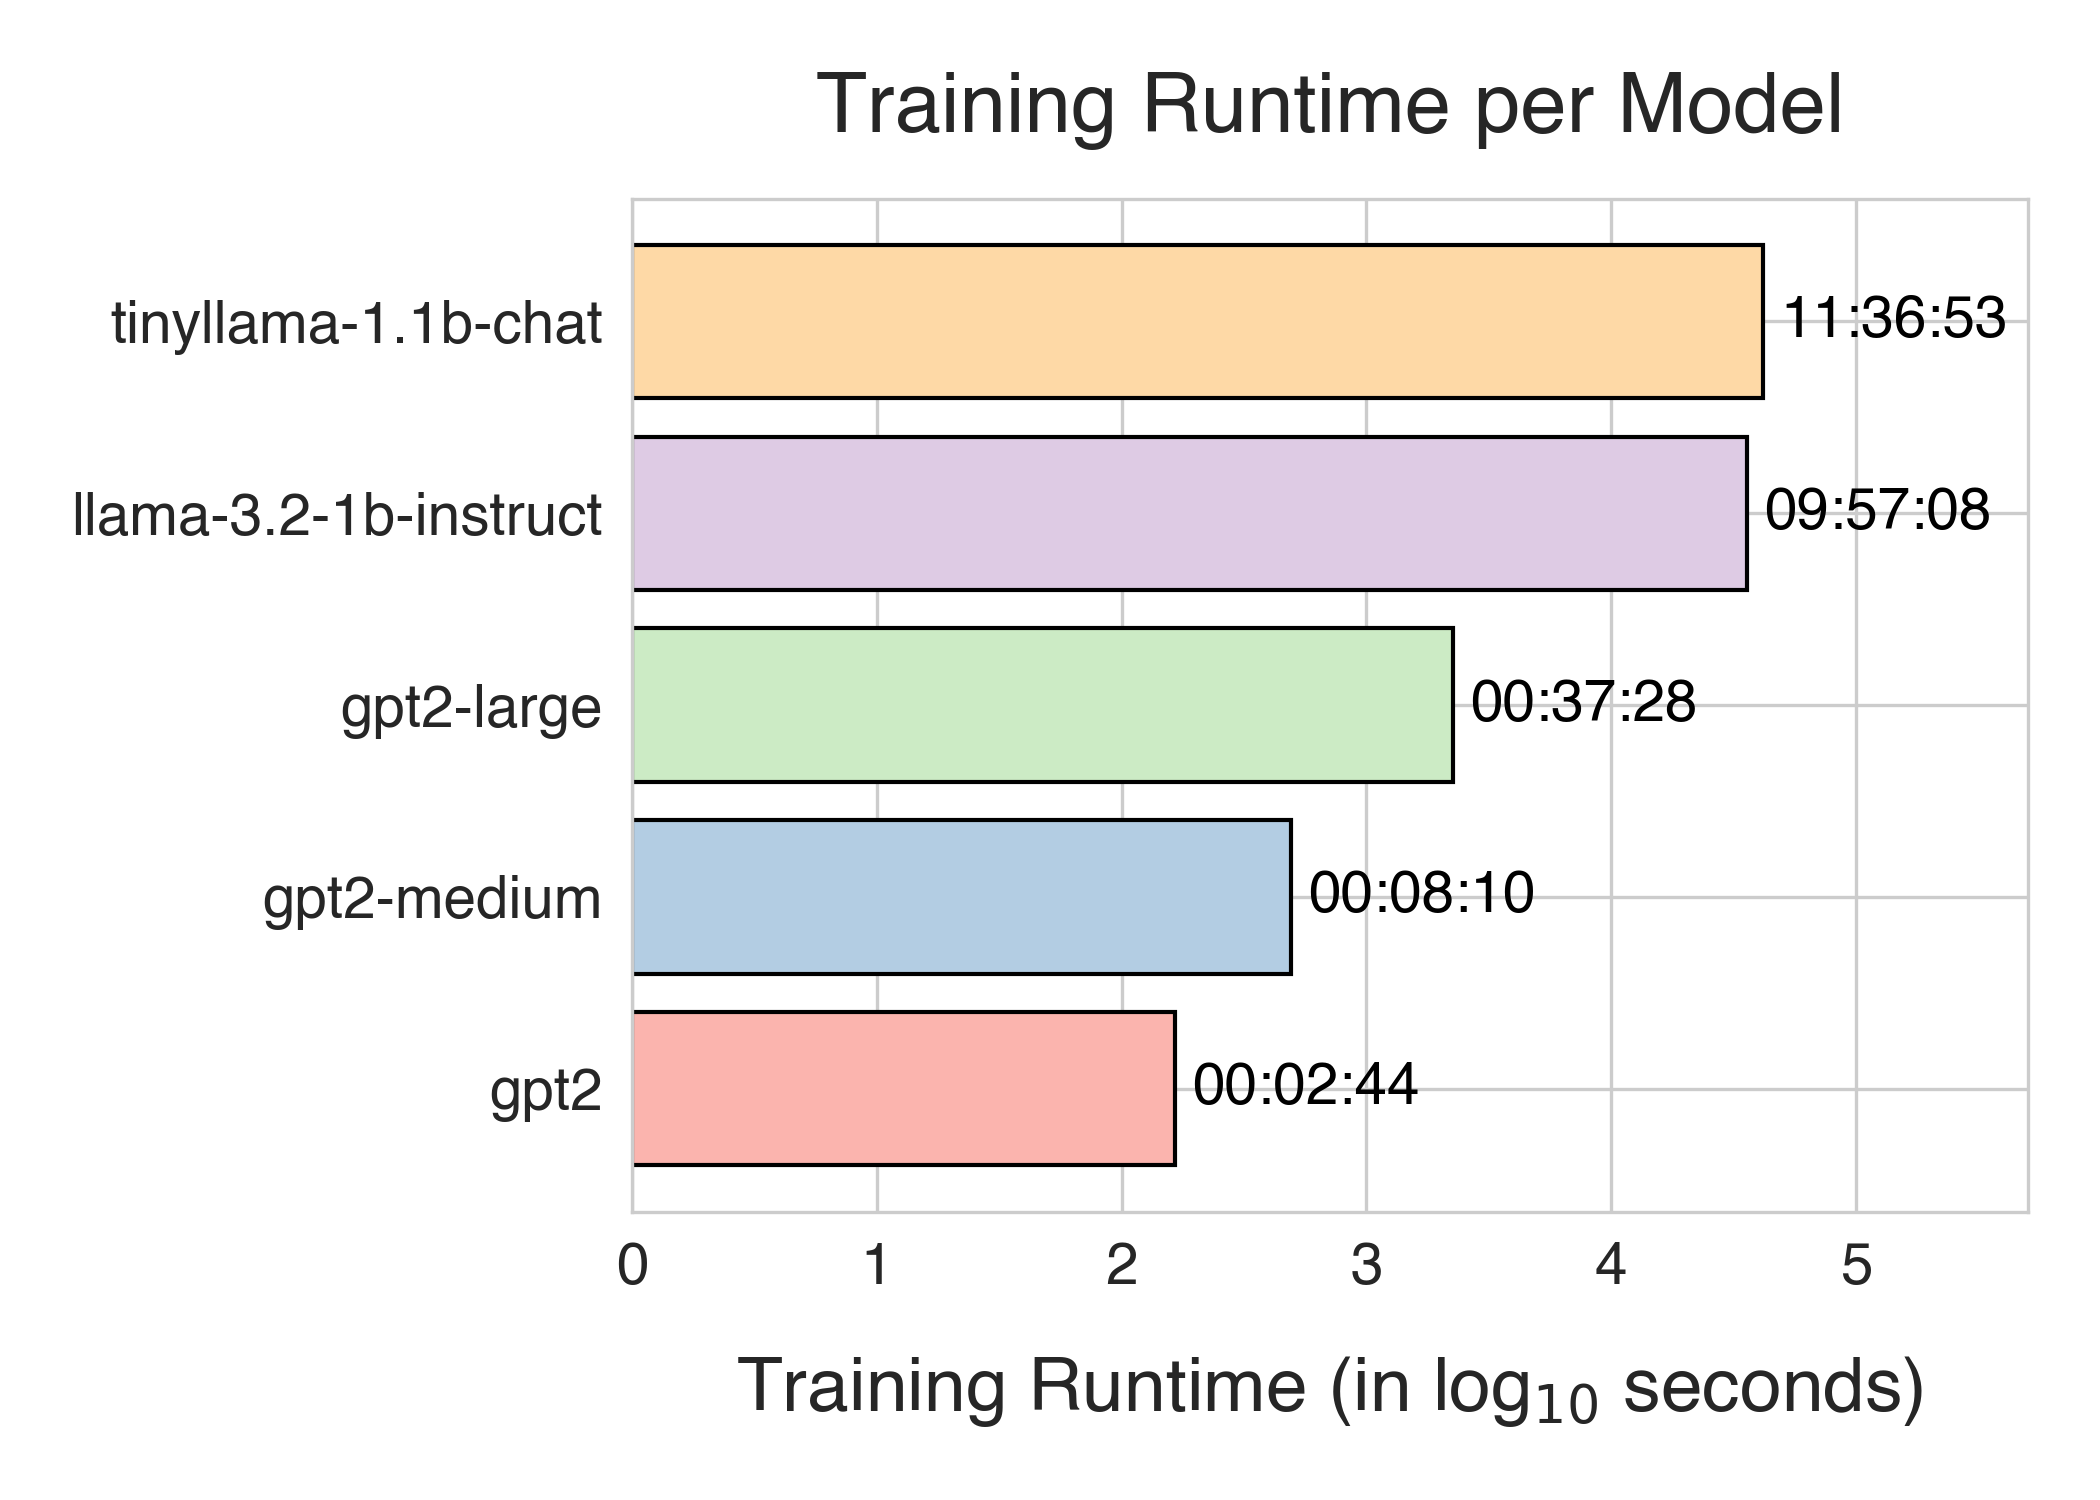
\includegraphics[width=\textwidth]{train_runtime.png}
    \caption{Training runtime (log scale). Bars show log-scaled durations in seconds; labels denote exact times per model.}
    \label{fig:runtime}
  \end{subfigure}
  \caption{Training diagnostics for fine-tuned models. The plots display loss progression, gradient norm stability, and overall training time, offering insight into optimization dynamics and efficiency.}
  \label{fig:training-diagnostics}
\end{figure}

The training phase across all models was conducted over a single epoch, with progressive
learning rate schedules and full logging of loss and gradient metrics. This section outlines
the training behavior and convergence characteristics observed during fine-tuning.

All models demonstrated a clear downward trend in training loss, reflecting consistent
optimization progress. GPT-2 Large showed the steepest decline, ending with a final
training loss of 1.6781, while TinyLLaMA-1.1B-Chat achieved the lowest overall value at
1.3555. In contrast, the base GPT-2 model plateaued around 2.4868, suggesting underfitting
relative to the other models.

Evaluation loss values followed a similar trend, with TinyLLaMA again achieving the
best result at 1.268, followed by GPT-2 Large at 1.523 and GPT-2 Medium at 1.882. These
results affirm that lower training loss generally correlated with stronger generalization to the
held-out evaluation data.

Gradient norms provide insight into training stability. GPT-2 and GPT-2 Medium
maintained stable and relatively low gradients (around 0.3-0.6), indicating smooth learning
curves. In contrast, TinyLLaMA exhibited initially high gradient norms (up to 2.5)
which steadily decreased, suggesting rapid adaptation followed by convergence. This steep
early learning curve likely contributed to its superior generalization performance.

The learning rate schedule, linearly increasing from 3e-6 to 3e-5, facilitated effective
warm-up across all models. No instabilities such as gradient explosions or sudden loss
spikes were observed, confirming the suitability of the chosen training configuration for
single-epoch fine-tuning.

In general, the training performance aligns with the evaluation results: models that
trained more efficiently and achieved lower losses also performed better on generation
metrics. Additionally, the findings suggest that smaller, modern architectures such as
TinyLLaMA can utilize compact parameterization for efficient fine-tuning while maintaining
high output quality.

\section{Quantitative Evaluation Results}

\begin{table}[t]
  \centering
  \scriptsize
  \renewcommand{\arraystretch}{1.3}
  \begin{tabularx}{0.95\textwidth}{
    >{\raggedright\arraybackslash}p{5cm}
    >{\centering\arraybackslash}X
    >{\centering\arraybackslash}X
    >{\centering\arraybackslash}X
    >{\centering\arraybackslash}X
  }
    \toprule
    \textbf{Model} & \textbf{Perplexity} & \textbf{BLEU} & \textbf{METEOR} & \textbf{F1} \\
    \midrule
    GPT-2 & 8.65 & 0.0221 & 0.2414 & 0.7883 \\
    GPT-2 Medium & 6.57 & 0.0242 & \textbf{0.2544} & 0.7921 \\
    GPT-2 Large & 4.59 & 0.0266 & 0.2297 & 0.7862 \\
    LLaMA-3.2-1B-Instruct & 5.34 & 0.0256 & 0.2377 & 0.7857 \\
    TinyLLaMA-1.1B-Chat-v1.0 & \textbf{3.56} & \textbf{0.0307} & 0.2184 & \textbf{0.7879} \\
    \bottomrule
  \end{tabularx}
  \caption{Detailed quantitative evaluation results for each fine-tuned model}
  \label{table:quant-results}
\end{table}

\begin{figure}[t]
  \centering
  \begin{subfigure}[t]{0.48\textwidth}
    \centering
    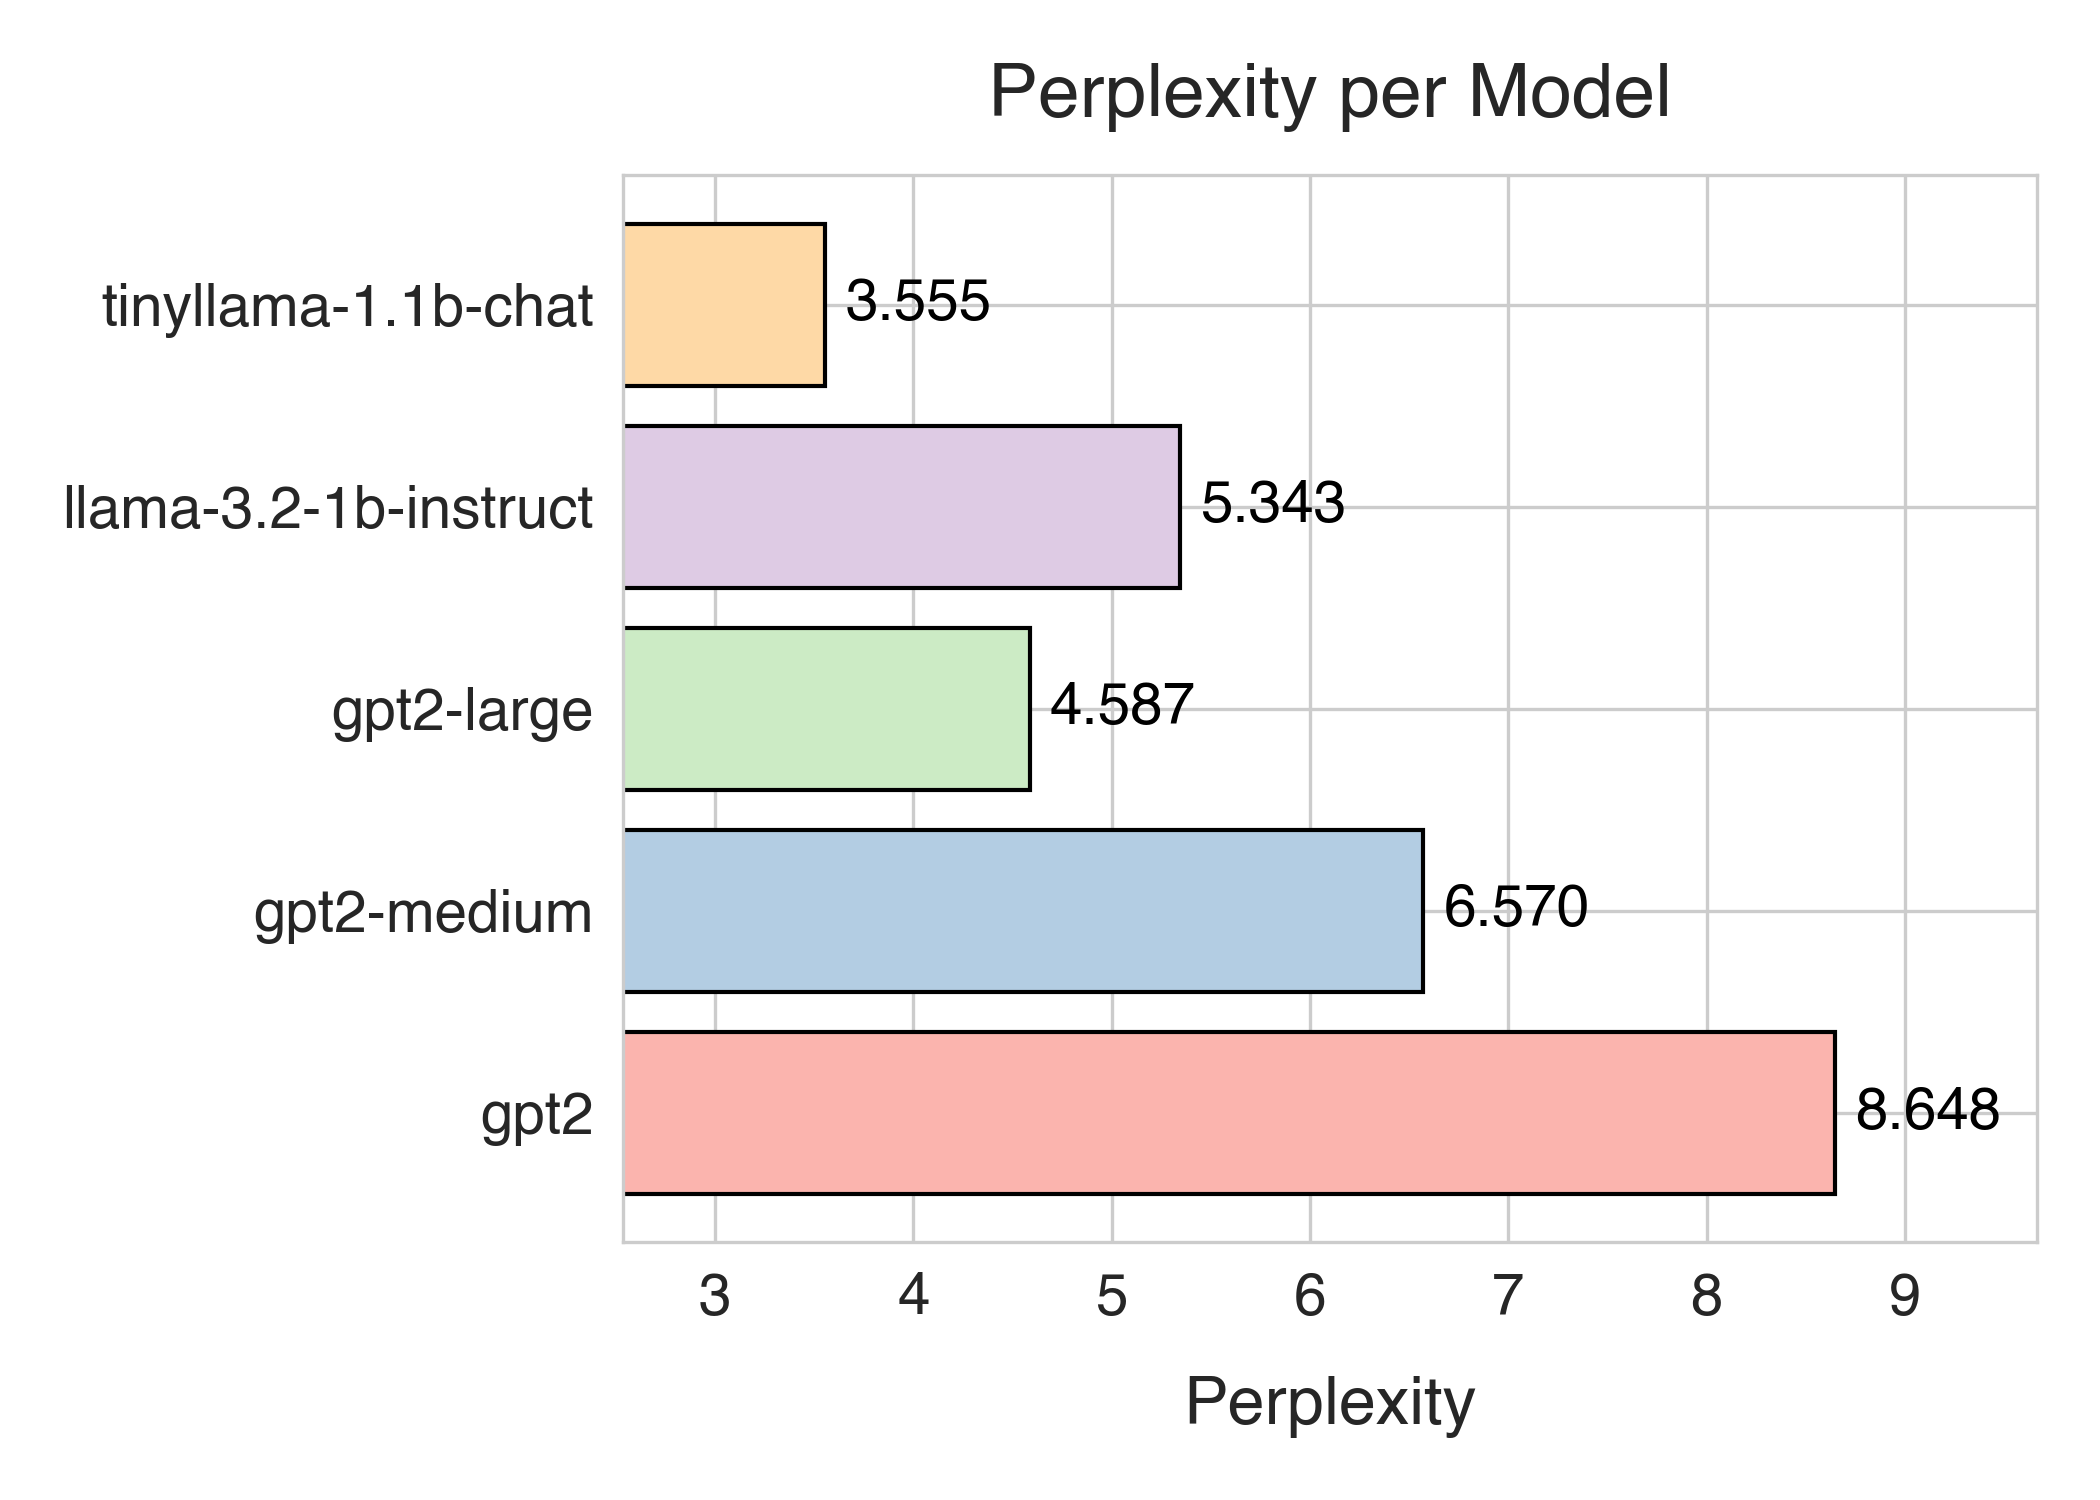
\includegraphics[width=\textwidth]{generation_perplexity.png}
    \caption{Perplexity scores after fine-tuning. Lower values indicate better language modeling ability.}
    \label{fig:perplexity}
  \end{subfigure}
  \hfill
  \begin{subfigure}[t]{0.48\textwidth}
    \centering
    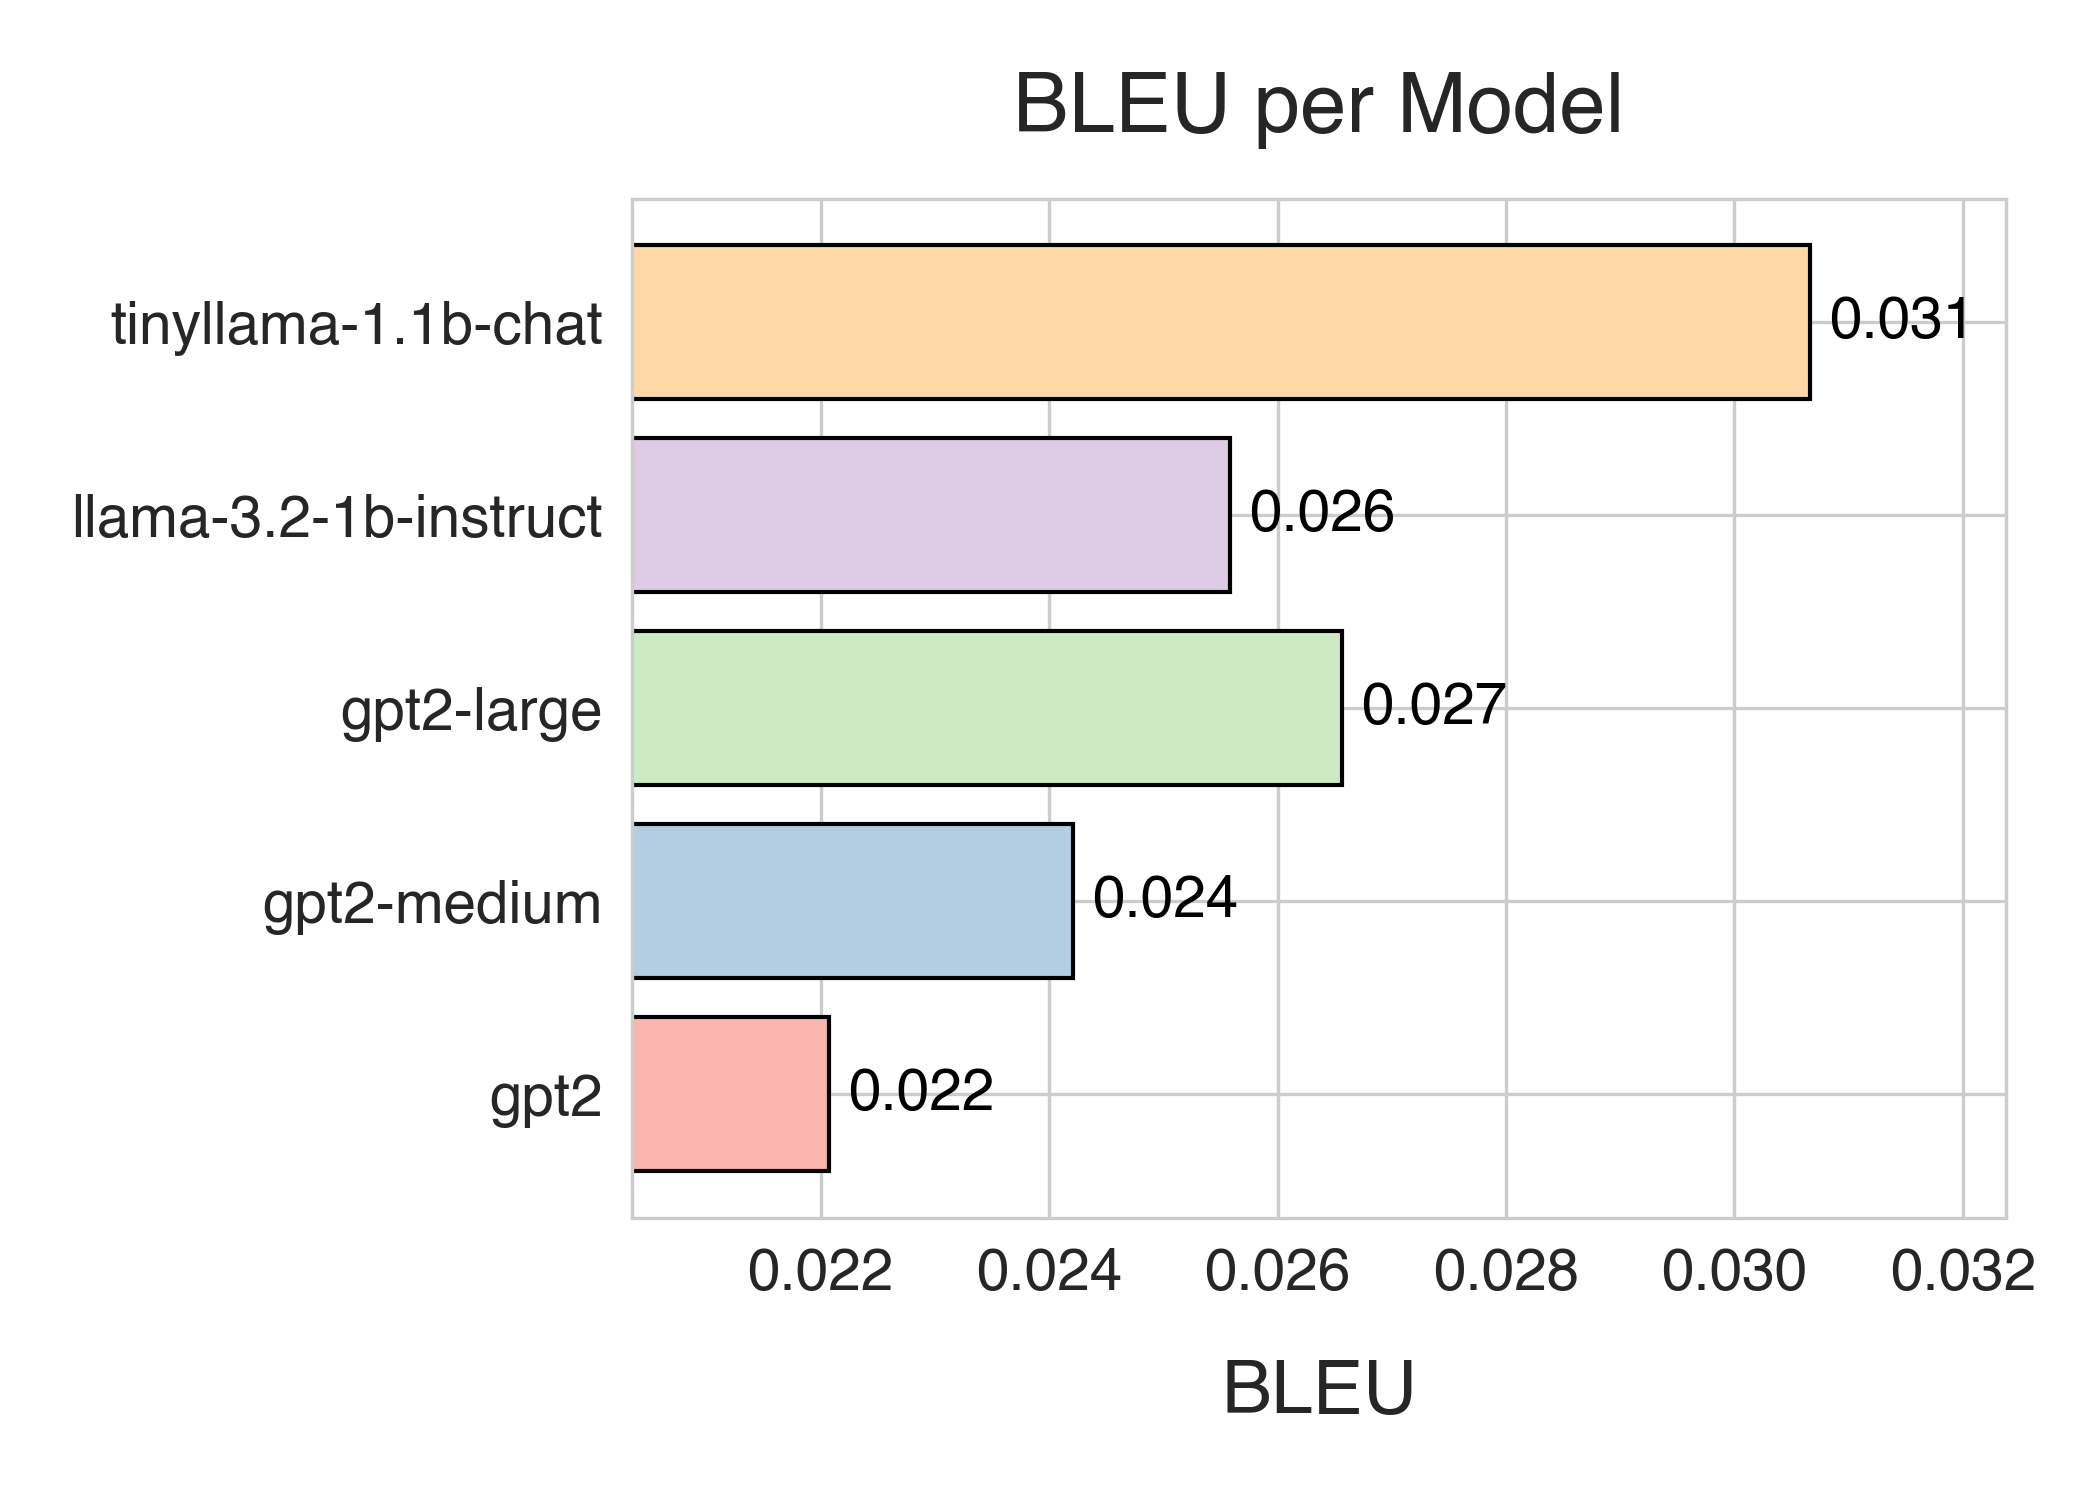
\includegraphics[width=\textwidth]{generation_bleu.png}
    \caption{BLEU scores of generated quests. Higher scores reflect stronger lexical overlap with references.}
    \label{fig:bleu}
  \end{subfigure}
  \vskip\baselineskip
  \begin{subfigure}[t]{0.48\textwidth}
    \centering
    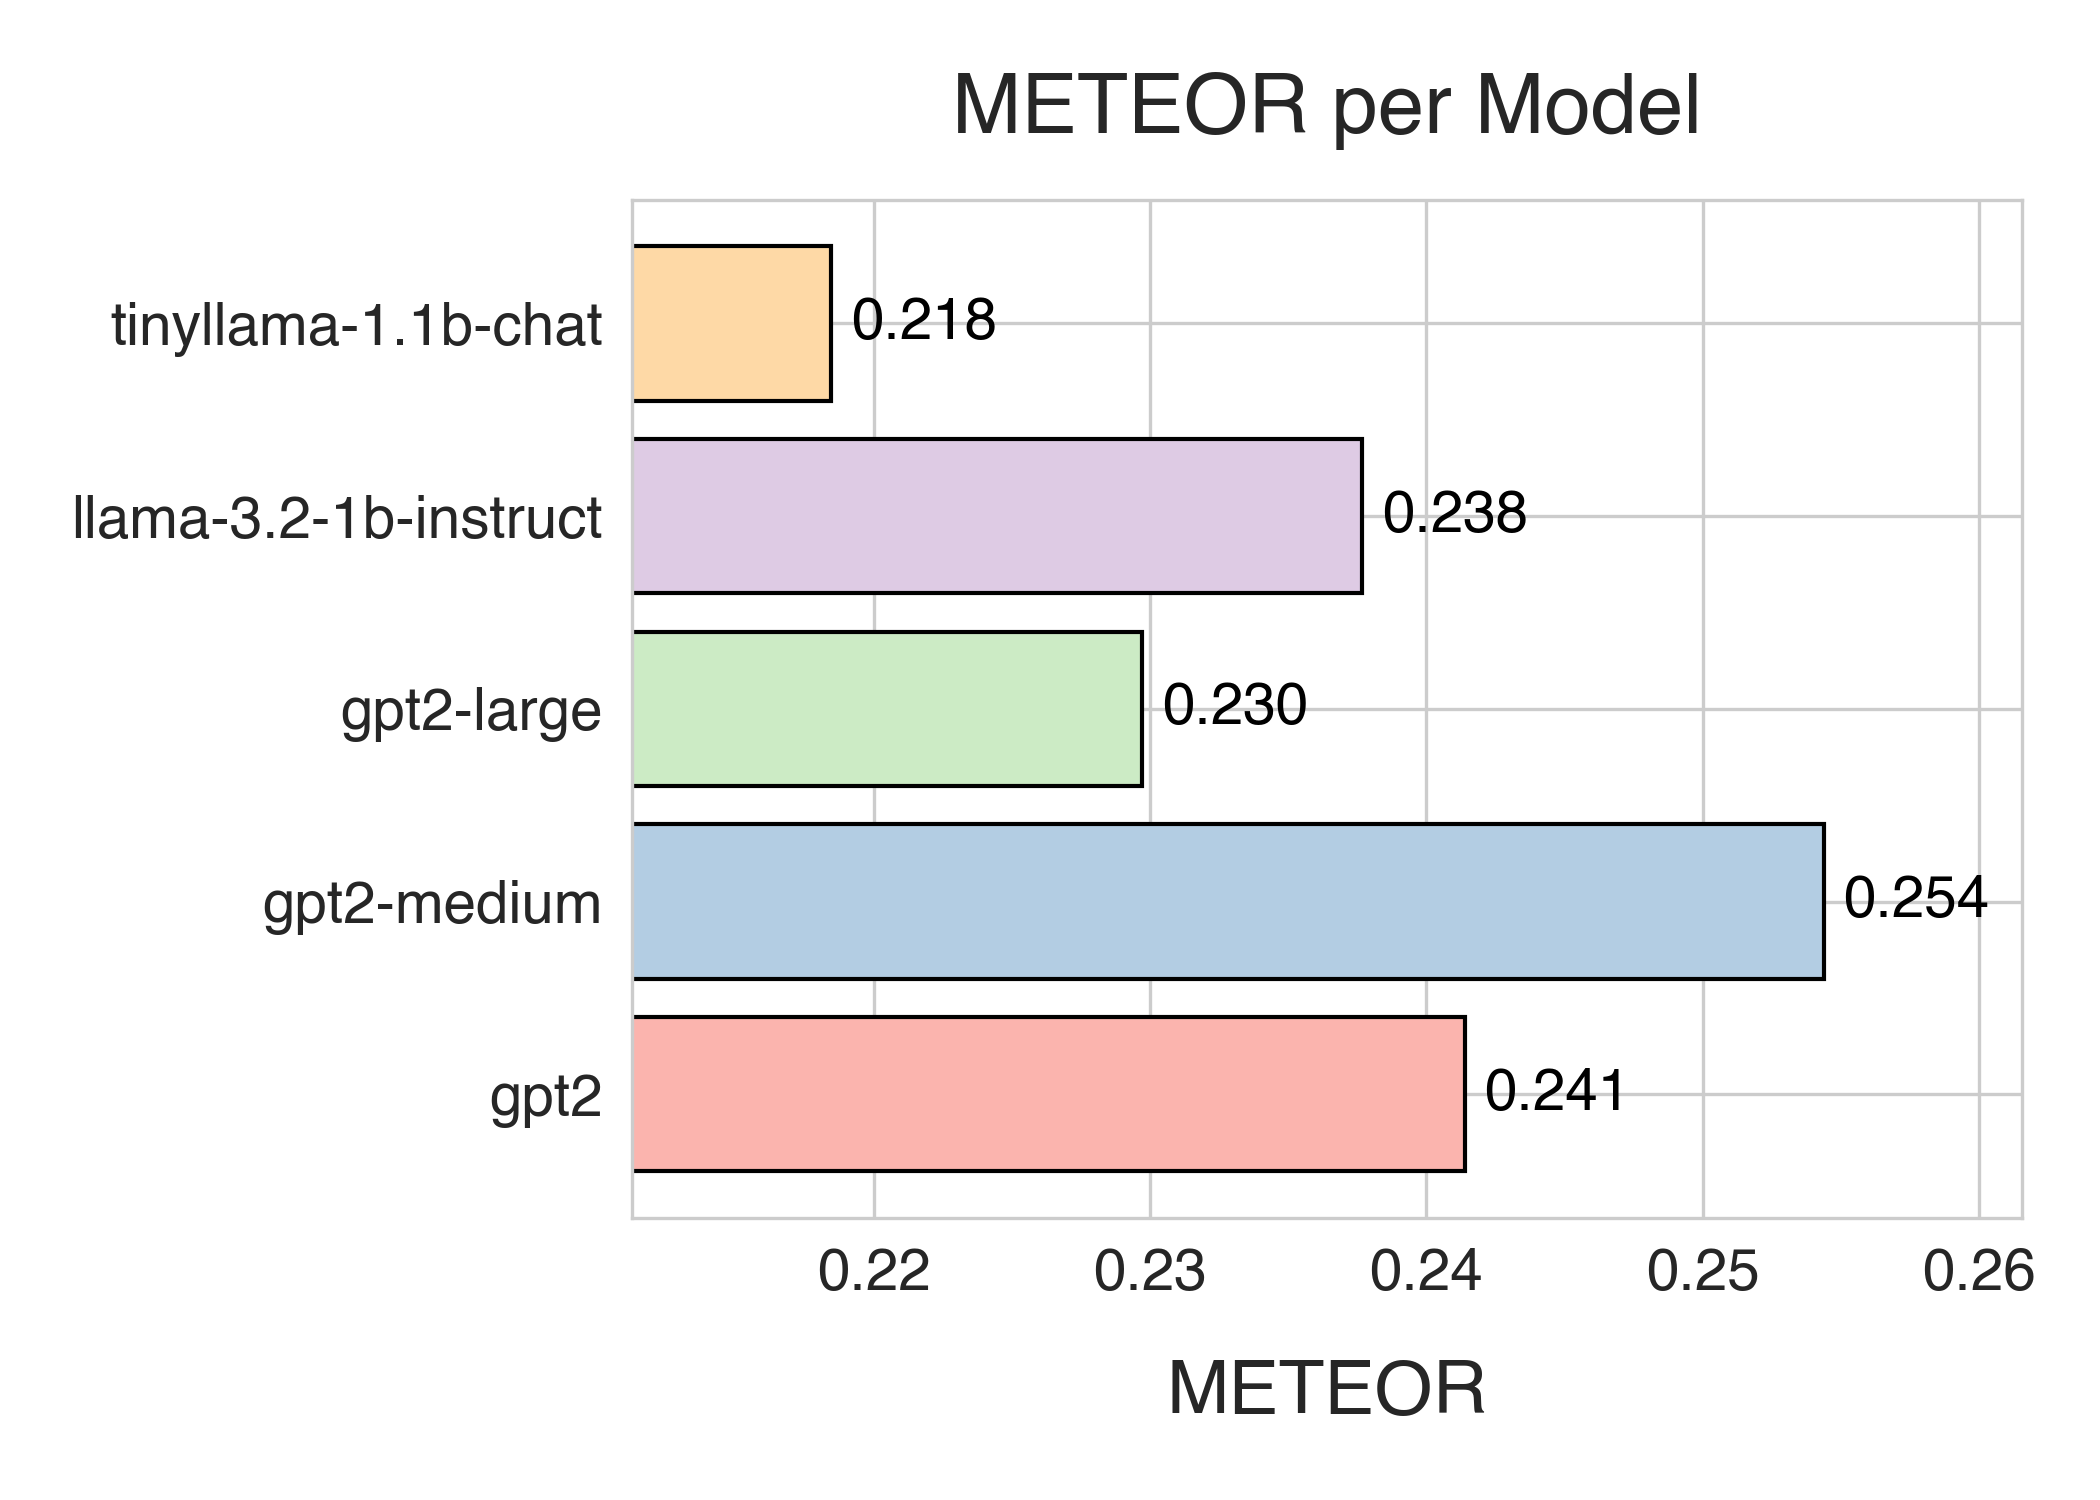
\includegraphics[width=\textwidth]{generation_meteor.png}
    \caption{METEOR scores, incorporating synonymy and stemming. Higher values indicate better semantic alignment.}
    \label{fig:meteor}
  \end{subfigure}
  \hfill
  \begin{subfigure}[t]{0.48\textwidth}
    \centering
    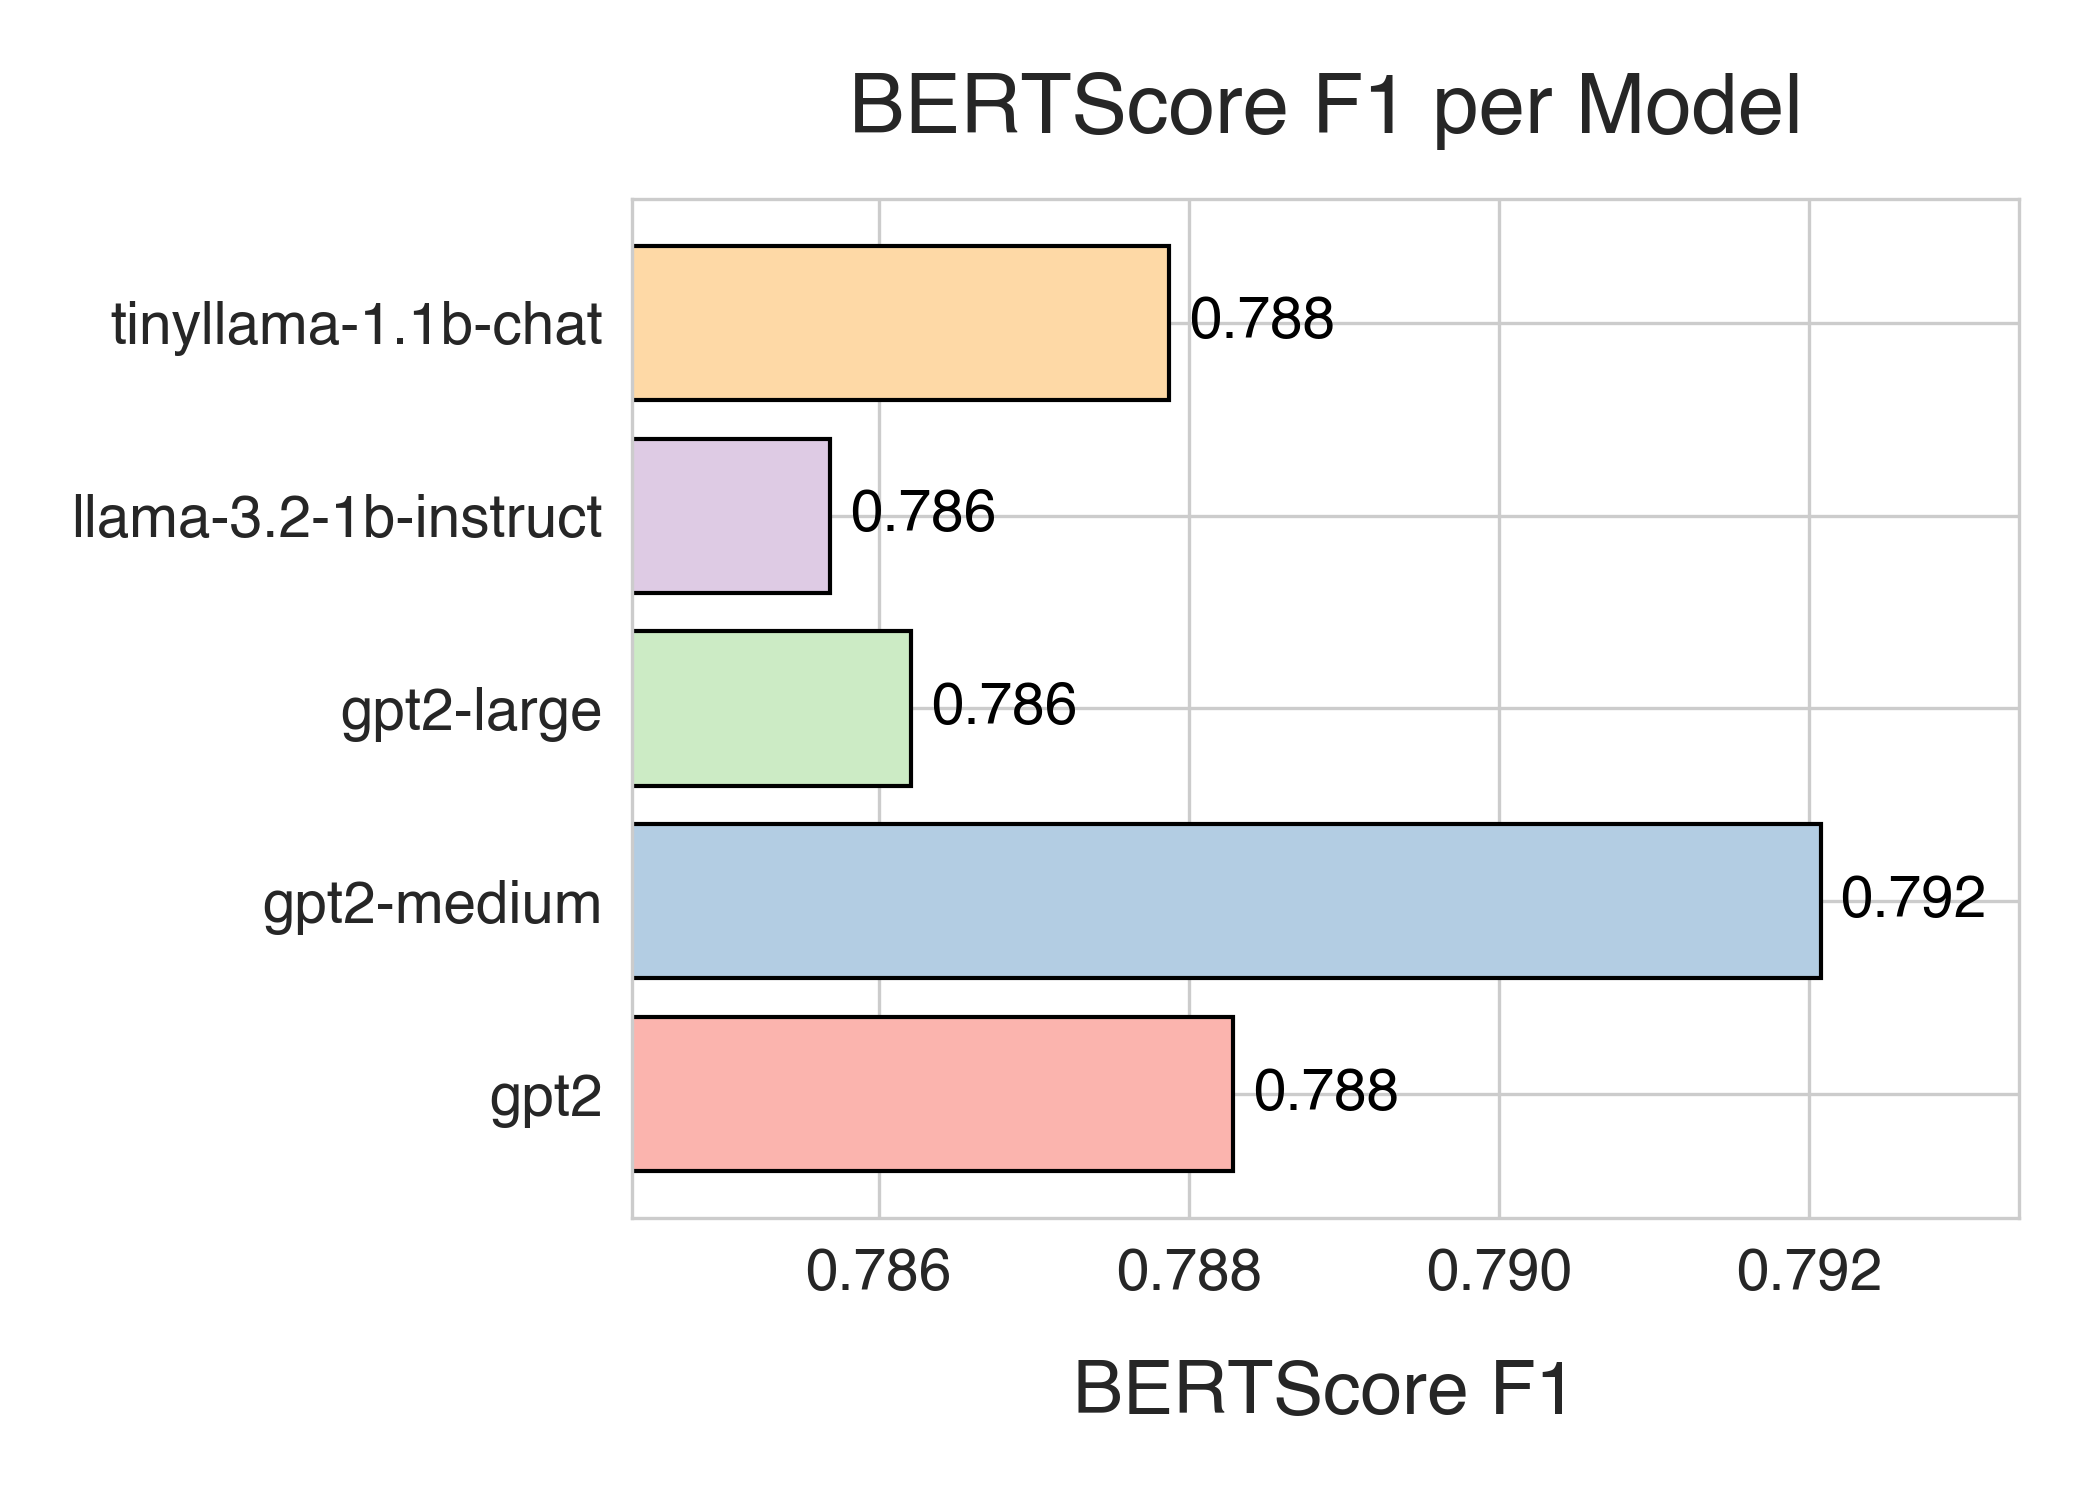
\includegraphics[width=\textwidth]{generation_bertscore.png}
    \caption{BERTScore F1 scores. Measures contextual semantic similarity using transformer embeddings.}
    \label{fig:bertscore}
  \end{subfigure}
  \caption{Automated evaluation results across models. The plots illustrate language modeling quality (Perplexity) and output similarity with reference quests using BLEU, METEOR, and BERTScore.}
  \label{fig:evaluation-metrics}
\end{figure}

Building on the hypothesis from related work~\cite{van2021fine}, which suggests that the GPT-2 and
the LLaMA pretraining dataset lacks a sufficient number of quest examples for high-quality
quest generation, we aimed to address this limitation through fine-tuning on a
specialized dataset.

Following the completion of fine-tuning and text generation, we evaluated model
performance using a suite of automatic metrics: Perplexity, BLEU, METEOR, and
BERTScore. These were chosen to capture various dimensions of output quality, such
as fluency, lexical overlap with reference texts, and semantic similarity. To ensure consistency
across model comparisons, all generations were produced using identical text
generation settings, including prompt structure, sampling strategies, and maximum sequence
lengths, as described in Section~\ref{section:text-generation-settings}.

By applying these metrics to both GPT-2 and LLaMA models with their increasing
sizes, we aim to quantify the improvements attributable to domain-specific learning.
Moreover, these quantitative evaluations form the basis for further model comparisons,
allowing us to investigate how architecture type, parameter scale, and fine-tuning strategy
contribute to performance in structured narrative generation tasks. Results are reported
in Table~\ref{table:quant-results} and are further analyzed in the following sections.

The quantitative evaluation results offer clear insights into the effectiveness of fine-tuning
for quest generation. Perplexity, a measure of language model confidence, was lowest
for TinyLLaMA 1.1B Chat (3.56), indicating its strong capability in producing
coherent, fluent outputs. This suggests that smaller instruction-tuned models, when fine-tuned
properly, can generalize effectively to domain-specific tasks.

In terms of BLEU, which assesses n-gram overlap with reference text, TinyLLaMA
again led with a score of 0.0307. This reflects its strength in mimicking the syntactic
structure of expected quest outputs. However, GPT-2 Large and LLaMA 3.2-1B also
performed competitively, indicating that larger models retain reasonable generalization
post fine-tuning.

Interestingly, GPT-2 Medium achieved the highest METEOR score (0.2544), which
evaluates semantic alignment and linguistic variation. This suggests that it captures the
meaning and phrasing of quests more effectively than other models. Meanwhile, TinyLLaMA
achieved the best BERTScore F1 (0.7879), indicating strong contextual similarity
between generated and reference quests.

These results validate our hypothesis that pretraining alone is insufficient for high-quality
quest generation. Fine-tuning on a structured dataset significantly boosts performance
across metrics. Notably, each model exhibits different strengths—TinyLLaMA
in fluency and structure, GPT-2 Medium in semantic coherence—implying that model
selection should align with specific generation goals.

\section{Discussion}

The results of this study demonstrate that fine-tuning LLMs on structured, domain-specific
quest data yields substantial improvements in both generation quality and model
convergence. Across evaluation and training metrics, clear patterns emerge that highlight
the effectiveness of targeted adaptation for PCG in RPGs.

From an evaluation standpoint, models such as TinyLLaMA-1.1B-Chat, GPT-2 Large,
and GPT-2 Medium consistently achieved higher scores across most metrics. TinyLLaMA
stood out with the best performance on BLEU, ROUGE, and BERTScore, indicating
strong lexical overlap and semantic similarity with ground truth references. While GPT-2
Medium showed slightly lower lexical overlap in BLEU, it achieved the highest METEOR
score, suggesting better handling of synonymy and paraphrasing. These results support
the hypothesis that larger models or more modern architectures can better model the
structured linguistic features of quests, especially when fine-tuned on relevant data.

Training dynamics also reflect this trend. All models demonstrated decreasing training
and evaluation losses across the single-epoch run, with TinyLLaMA achieving the lowest
evaluation loss (1.268), followed by GPT-2 Large (1.523) and LLaMA-3.2-1B-Instruct
(1.676). This loss reduction was accompanied by stable learning rate schedules and manageable
gradient norms. While TinyLLaMA initially exhibited high gradient norms, these
values decreased over time, indicating effective adaptation. In contrast, GPT-2 variants
displayed smooth and stable training trajectories with consistent learning progress.

The alignment between evaluation metrics and training loss suggests that models with
lower validation loss typically produced more semantically accurate and fluent quests.
Importantly, the high performance of TinyLLaMA—despite its relatively small parameter
count—demonstrates that smaller models, when fine-tuned effectively, can compete with
or surpass larger ones on domain-specific tasks. This highlights their potential for use in
real-time or resource-constrained game development environments.

Compared to the experiments conducted by V{\"a}rtinen et al.~\cite{vartinen2022generating}, which reported issues
such as overfitting, inconsistent handling of entities, and incomplete coverage of
quest elements, the models evaluated in this study exhibited more stable training behavior
and stronger alignment with target outputs. While the earlier work noted that the
larger GPT-2 variant outperformed its smaller counterpart in coherence and coverage, this
study finds similar trends, with larger or more recent models like TinyLLaMA and GPT-2 Large
achieving higher scores across multiple evaluation metrics. Additionally, although
the reference study observed higher perplexity with XML-like formats, the prompt-aligned
structure used here did not appear to negatively impact model performance. These findings
suggest that model architecture, fine-tuning configuration, and prompt design all play
important roles in shaping the quality and consistency of generated quests, particularly
in domain-specific contexts.

In summary, the experiments validate the role of fine-tuning in enhancing LLM performance
on PQG. Both quantitative metrics and training behavior confirm that adaptation
enables models to better internalize structural patterns, narrative conventions,
and content constraints of the RPG domain. These findings lay a strong foundation for further
research involving longer training schedules, multi-turn dialogue integration, or hybrid
systems incorporating symbolic planners and knowledge graphs~\cite{ashby2023personalized}.

\newpage
